\documentclass[a4paper,openany]{book} 
\usepackage{bm}
\usepackage{cmap}
\usepackage{ctex}
\usepackage{cite}
\usepackage{color}
\usepackage{float}
\usepackage{xeCJK}
\usepackage{amsthm}
\usepackage{amsmath}
\usepackage{amssymb}
\usepackage{setspace}
\usepackage{geometry}
\usepackage{hyperref}
\usepackage{enumerate}
\usepackage{indentfirst}
\usepackage{yfonts}
\usepackage{pdfpages}

\usepackage[cache=false]{minted}

%代码高亮
\geometry{margin=1in}

\newcommand{\cppcode}[1]
{
  \inputminted[mathescape,
  tabsize=4,
  linenos,
  framesep=2mm,
  breakaftergroup=true,
  breakautoindent=true,
  breakbytoken=true,
  breaklines=true,
  fontsize=\small
  ]{cpp}{Source/#1}
}

\newcommand{\javacode}[1]
{
  \inputminted[mathescape,
  tabsize=4,
  linenos,
  framesep=2mm,
  breakaftergroup=true,
  breakautoindent=true,
  breakbytoken=true,
  breaklines=true,
  fontsize=\small
  ]{java}{Source/#1}
}

\newcommand{\emacscode}[1]
{
  \inputminted[mathescape,
  tabsize=4,
  linenos,
  % frame=single,
  framesep=2mm,
  breakaftergroup=true,
  breakautoindent=true,
  breakbytoken=true,
  breaklines=true,
  fontsize=\small
  ]{emacs}{Source/#1}
}

\title{\Huge\textgoth{Code Library for Lmxyy\thanks{https://github.com/lmxyy/Code-Library-for-Lmxyy} \\Version 2.0}}
\author{Lmxyy \\ \emph{Shanghai Jiao Tong University}}
\date{\today}
\begin{document}
\maketitle
\newpage
\newpage
\tableofcontents
\newpage

\chapter{Algorithms}
\section{1D1D Dynamic Programming}
\cppcode{Algorithms/1D1D Dynamic Programming.cpp}
\section{Dynamic Minimal Spanning Tree}
\cppcode{Algorithms/Dynamic Minimal Spanning Tree.cpp}
\section{Plug-like Dynamic Programming}
\cppcode{Algorithms/Plug-like Dynamic Programming.cpp}
\section{Slop Optimization}
\cppcode{Algorithms/Slop Optimization.cpp}
\section{Three-dimension Partial Order}
\cppcode{Algorithms/Three-dimension Partial Order.cpp}

\chapter{Computational Geometry}
\section{Circle Intersection}
\cppcode{Computational Geometry/Circle Intersection.cpp}
\section{Common Formulas}
\cppcode{Computational Geometry/Common Formulas.cpp}
\section{Convex Hull}
\cppcode{Computational Geometry/Convex Hull.cpp}
\section{Cross Points of Circles}
\cppcode{Computational Geometry/Cross Points of Circles.cpp}
\section{Cross Points of Line and Circle}
\cppcode{Computational Geometry/Cross Points of Line and Circle.cpp}
\section{Graham Scanning Algorithm}
\cppcode{Computational Geometry/Graham Scanning Algorithm.cpp}
\section{Half Plane Intersection}
\cppcode{Computational Geometry/Half Plane Intersection.cpp}
\section{Intersecting Area of Circle and Polygon}
\cppcode{Computational Geometry/Intersecting Area of Circle and Polygon.cpp}
\section{Intersection of Line and Convex Hull}
\cppcode{Computational Geometry/Intersection of Line and Convex Hull.cpp}
\section{Minimal Product}
\cppcode{Computational Geometry/Minimal Product.cpp}
\section{Planar Graph}
\cppcode{Computational Geometry/Planar Graph.cpp}
\section{Polygon Class}
\cppcode{Computational Geometry/Polygon Class.cpp}
\section{Union Area of Circles}
\cppcode{Computational Geometry/Union Area of Circles.cpp}

\chapter{Data Structure}
\section{Divide and Conquer on Tree}
\cppcode{/Data Structure/Divide and Conquer on Tree.cpp}
\section{Dynamicly Divide and Conquer on Tree}
\cppcode{/Data Structure/Dynamicly Divide and Conquer on Tree.cpp}
\section{Heavy Path Decomposition}
\cppcode{/Data Structure/Heavy Path Decomposition.cpp}
\section{K-Dimension Tree}
\cppcode{/Data Structure/K-Dimension Tree.cpp}
\section{Leftlist Tree}
\cppcode{/Data Structure/Leftlist Tree.cpp}
\section{Link Cut Tree}
\cppcode{/Data Structure/Link Cut Tree.cpp}
\section{Merge Split Treap}
\cppcode{/Data Structure/Merge Split Treap.cpp}
\section{Modui Algorithm on Tree}
\cppcode{/Data Structure/Modui Algorithm on Tree.cpp}
\section{Modui Algorithm without Deletion}
\cppcode{/Data Structure/Modui Algorithm without Deletion.cpp}
\section{President Tree}
\cppcode{/Data Structure/President Tree.cpp}
\section{Splay}
\cppcode{/Data Structure/Splay.cpp}

\chapter{Graph Theory}
\section{2-Sat}
\cppcode{/Graph Theory/2-Sat.cpp}
\section{Bridges and Cut Vertices}
\cppcode{/Graph Theory/Bridges and Cut Vertices.cpp}
\section{Cost Flow}
\cppcode{/Graph Theory/Cost Flow.cpp}
\section{Difference Constraints}
\cppcode{/Graph Theory/Difference Constraints.cpp}
\section{Dinic Algorithm}
\cppcode{/Graph Theory/Dinic Algorithm.cpp}
\section{Dominator Tree}
\cppcode{/Graph Theory/Dominator Tree.cpp}
\section{Hungary}
\cppcode{/Graph Theory/Hungary.cpp}
\section{Isap Algorithm}
\cppcode{/Graph Theory/Isap Algorithm.cpp}
\section{Kuhn-Munkres Algorithm}
\cppcode{/Graph Theory/Kuhn-Munkres Algorithm.cpp}
\section{Maximal Matching in General Graphs}
\cppcode{/Graph Theory/Maximal Matching in General Graphs.cpp}
\section{Maximal Weighted  Matching in General Graphs}
\cppcode{/Graph Theory/Maximal Weighted  Matching in General Graphs.cpp}
\section{Maximum Cardinality Search}
\cppcode{/Graph Theory/Maximum Cardinality Search.cpp}
\section{Network Flow with Lower Bound}
\begin{enumerate}[1.]
\item \textbf{无源汇有上下界可行流}
  
  设原来源点为$Source$,汇点是$Sink$。新建一个超级源$SuperSource$和超级汇$SuperSink$。对于原网络中的每一条边$u \rightarrow v$,上界$U$,下界$L$,将它拆分为三条边:
  \begin{enumerate}[(1)]
  \item $u \rightarrow SuperSink$,容量为$L$。
  \item $SuperSource \rightarrow v$,容量为$L$。
  \item $u \rightarrow v$,容量为$U-L$。
  \end{enumerate}
  最后添加边$Sink \rightarrow Source$,容量为$+\infty$。在新建的网络上,计算从$SuperSource$到$SuperSink$的最大流。若每条从$SuperSource$发出的边都满流,说明存在可行流,否则不。每条边实际流量为容量下界$+$附加流中它的流量。
\item \textbf{有源汇有上下界可行流}
  
  在``无源汇有上下界可行流''建图上,新增一条$Sink \rightarrow Source$的边,容量为$+\infty$即可。
\item \textbf{有源汇有上下界最大流}
  
  在``有源汇有上下界可行流''建图上,先判断是否存在可行流,若存在可行流,拆掉$Sink \rightarrow Source$的边后,接着在图中$Source \rightarrow Sink$最大流增广加上原可行流即为最大流答案。(若存在可行流,去掉下界后最大流即为原图有源汇有上下界最大流)
\item \textbf{有源汇有上下界最小流}
  
  在``有源汇有上下界可行流''建图上,先判断是否存在可行流,若存在可行流,拆掉$Sink \rightarrow Source$的边后,用可行流减去在图中$Sink \rightarrow Source$增广的最大流即为最小流答案。
\end{enumerate}

在实现时,可以吧$SuperSource$连向同一节点的多条边合成一条(容量合并。从同一节点指向$SuperSink$的多条边也应合并。

对于费用流,只需要改变将网络流算法改成费用流算法。对于原网络中的每一条边$u \rightarrow v$,上界$U$,下界$L$,费用$c$,将它拆分为三条边:
\begin{enumerate}[(1)]
\item $u \rightarrow SuperSink$,容量为$L$,费用$c$。
\item $SuperSource \rightarrow v$,容量为$L$,费用$0$。
\item $u \rightarrow v$,容量为$U-L$,费用$c$。
\end{enumerate}
\section{Point Biconnected Component}
\cppcode{/Graph Theory/Point Biconnected Component.cpp}
\section{Steiner Tree}
\cppcode{/Graph Theory/Steiner Tree.cpp}
\section{Stoer Wagner Algorithm}
\cppcode{/Graph Theory/Stoer Wagner Algorithm.cpp}
\section{Strongly Connected Component}
\cppcode{/Graph Theory/Strongly Connected Component.cpp}
\section{Virtual Tree}
\cppcode{/Graph Theory/Virtual Tree.cpp}
\section{Zhu-Liu Algorithm}
\cppcode{/Graph Theory/Zhu-Liu Algorithm.cpp}
\section{ZKW Cost Flow}
\cppcode{/Graph Theory/ZKW Cost Flow.cpp}

\chapter{Number Theory}
\section{Baby Step Giant Step}
\cppcode{/Number Theory/Baby Step Giant Step.cpp}
\section{Chinese Remainder Theorem}
\cppcode{/Number Theory/Chinese Remainder Theorem.cpp}
\section{Extended Euclidean Algorithm}
\cppcode{/Number Theory/Extended Euclidean Algorithm.cpp}
\section{Linearly Sieve}
\cppcode{/Number Theory/Linearly Sieve.cpp}
\section{N-Power Residue}
\cppcode{/Number Theory/N-Power Residue.cpp}
\section{Number Theoretic Transformation}
\cppcode{/Number Theory/Number Theoretic Transformation.cpp}
\section{Pollard Rho Algorithm}
\cppcode{/Number Theory/Pollard Rho Algorithm.cpp}
\section{Primitive Root}
\cppcode{/Number Theory/Primitive Root.cpp}
\section{Quadratic Residue}
\cppcode{/Number Theory/Quadratic Residue.cpp}
\section{Single Variable Modulus Linear Equation}
\cppcode{/Number Theory/Single Variable Modulus Linear Equation.cpp}

\chapter{Numerical Algorithms}
\section{Counting Integral Points under Straight Line}
\cppcode{/Numerical Algorithms/Counting Integral Points under Straight Line.cpp}
\section{Evaluation of Expression}
\cppcode{/Numerical Algorithms/Evaluation of Expression.cpp}
\section{Fast Fourier Transformation}
\cppcode{/Numerical Algorithms/Fast Fourier Transformation.cpp}
\section{Fast Input and Output}
\cppcode{/Numerical Algorithms/Fast Input and Output.cpp}
\section{Fraction Class}
\cppcode{/Numerical Algorithms/Fraction Class.cpp}
\section{Gray Code}
\cppcode{/Numerical Algorithms/Gray Code.cpp}
\section{Numerical Integration}
\cppcode{/Numerical Algorithms/Numerical Integration.cpp}
\section{Simplex}
\subsection{Description}
有$n$个实数变量$x_1,x_2,\ldots,x_n$和$m$条约束,其中第$i$条约束形如 $\sum_{i = 1}^{n}a_{i,j}x_j \leq b_i$。

此外这$n$个变量需要满足非负性限制,$x_j \geq 0$。

在满足上述所有条件的情况下,你需要指定每个变量$x_j$的取值,使得目标函数$F = \sum_{j = 1}^{n}c_jx_j$的值最大。

\subsection{Input}
第一行三个正整数$n,m,t$。其中$t \in \{ 0,1 \}$。

第二行有$n$个整数$c_1,c_2,\ldots,c_n$,整数间均用一个空格分隔。

接下来$m$行,每行代表一条约束,其中第$i$行有$n+1$个整数$a_{i1},a_{i2},\ldots,a_{in},b_i$,整数间均用一个空格分隔。
\subsection{Output}
如果不存在满足所有约束的解,仅输出一行``Infeasible''。

如果对于任意的$M$,都存在一组解使得目标函数的值大于$M$,仅输出一行``Unbounded''。

否则,第一行输出一个实数,表示目标函数的最大值$F$。

如果$t=1$,那么你还需要输出第二行,用空格隔开的$n$个非负实数,表示此时$x_1,x_2,\ldots,x_n$的取值,如有多组方案请任意输出其中一个。
\subsection{Code}
\cppcode{/Numerical Algorithms/Simplex.cpp}
\section{Solutions of Equation of Higher Order}
\cppcode{/Numerical Algorithms/Solutions of Equation of Higher Order.cpp}

\chapter{String Algorithms}
\section{Aho-Corasick Automaton}
\cppcode{/String Algorithms/Aho-Corasick Automaton.cpp}
\section{Extended Knuth-Morris-Pratt Algorithm}
\cppcode{/String Algorithms/Extended Knuth-Morris-Pratt Algorithm.cpp}
\section{Knuth-Morris-Pratt Algorithm}
\cppcode{/String Algorithms/Knuth-Morris-Pratt Algorithm.cpp}
\section{Manacher Algorithm}
\cppcode{/String Algorithms/Manacher Algorithm.cpp}
\section{Palindrome Automaton}
\cppcode{/String Algorithms/Palindrome Automaton.cpp}
\section{Suffix Array}
\cppcode{/String Algorithms/Suffix Array.cpp}
\section{Suffix Automaton}
\cppcode{/String Algorithms/Suffix Automaton.cpp}

\chapter{Others}
\section{Calculation of Date}
\cppcode{/Others/Calculation of Date.cpp}
\section{Java Hints}
\subsection{Code Example}
\javacode{/Others/Java Hints/Code.java}
\subsection{Class Reference}
\subsubsection{BigDecimal Class}
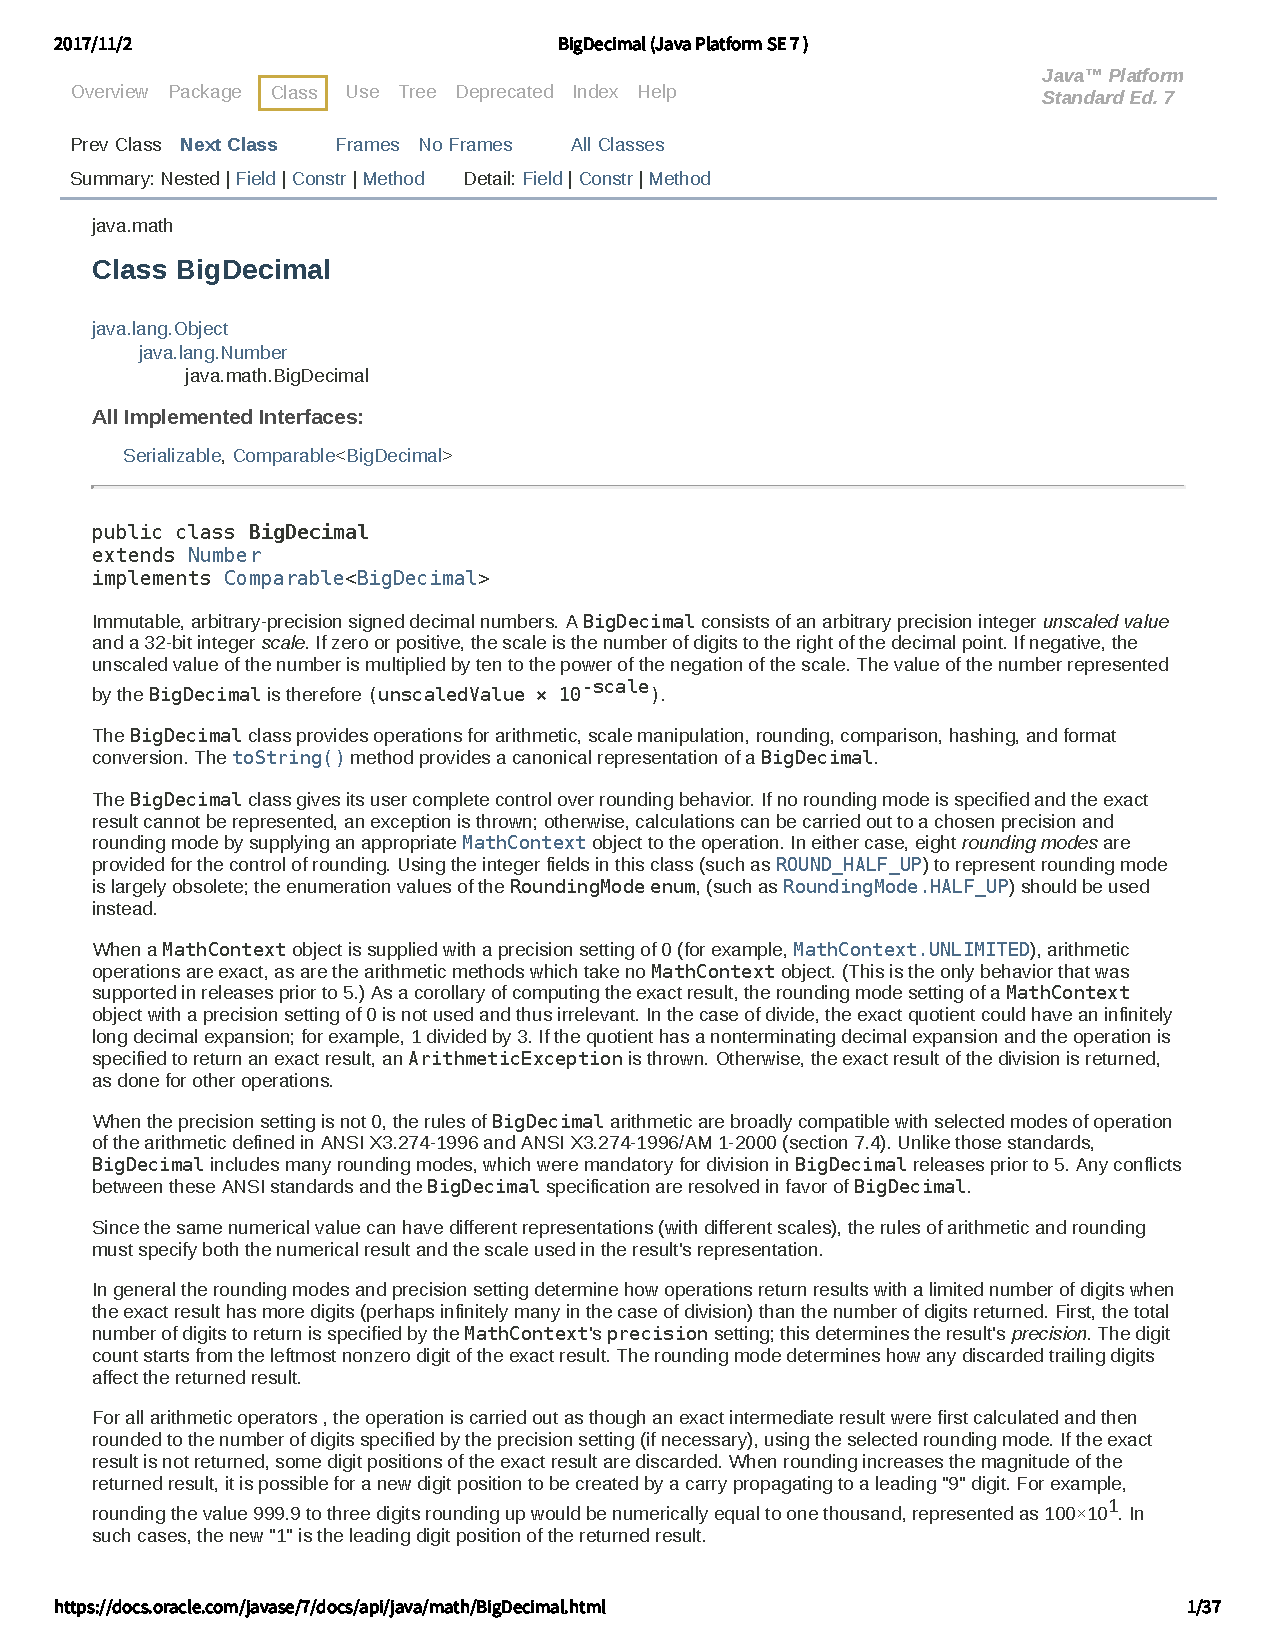
\includepdf[scale = 0.8,pages=1-7,pagecommand = {}]{BigDecimal-Class.pdf}
\newpage
% \subsubsection{BigInteger Class}
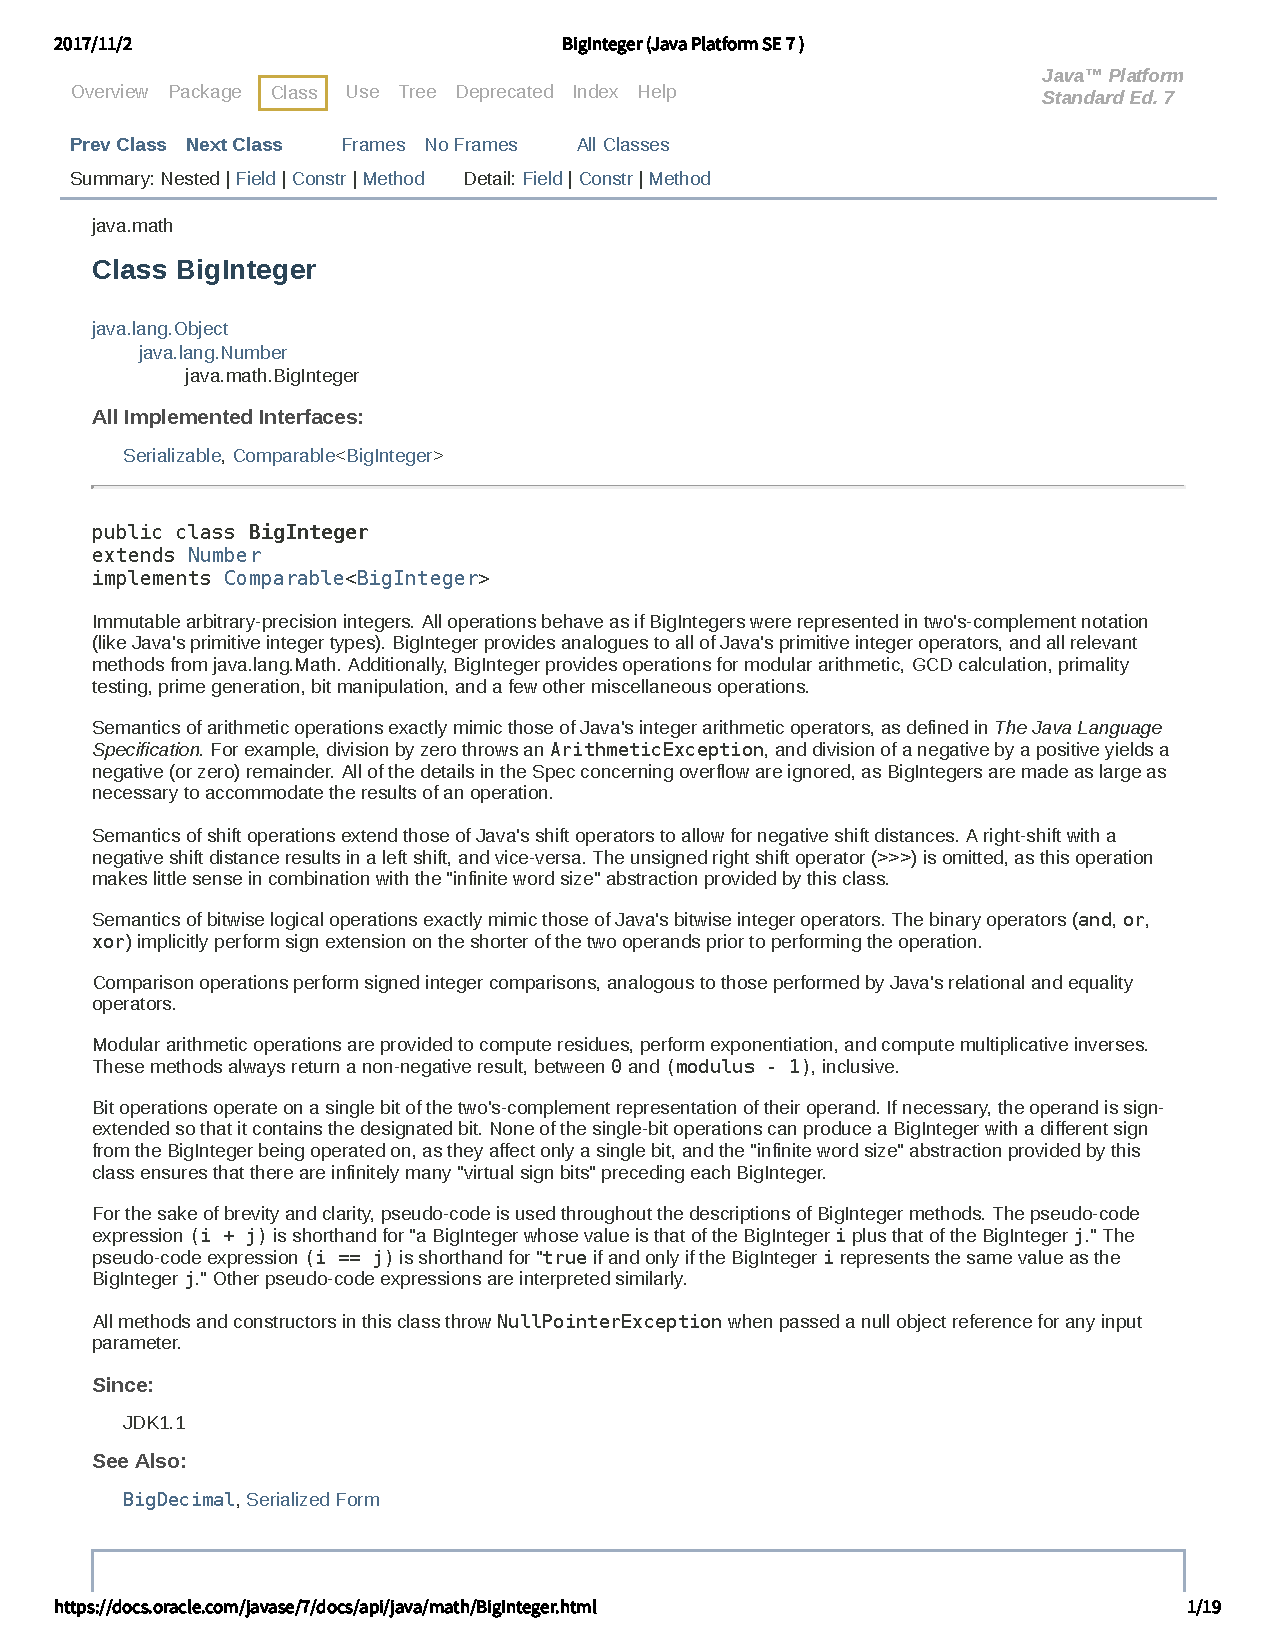
\includepdf[scale = 0.8,pages=1,pagecommand = \subsubsection{BigInteger Class}]{BigInteger-Class.pdf}
\includepdf[scale = 0.8,pages=2-4,pagecommand = {}]{BigInteger-Class.pdf}
\newpage
% \subsubsection{MathContext Class}
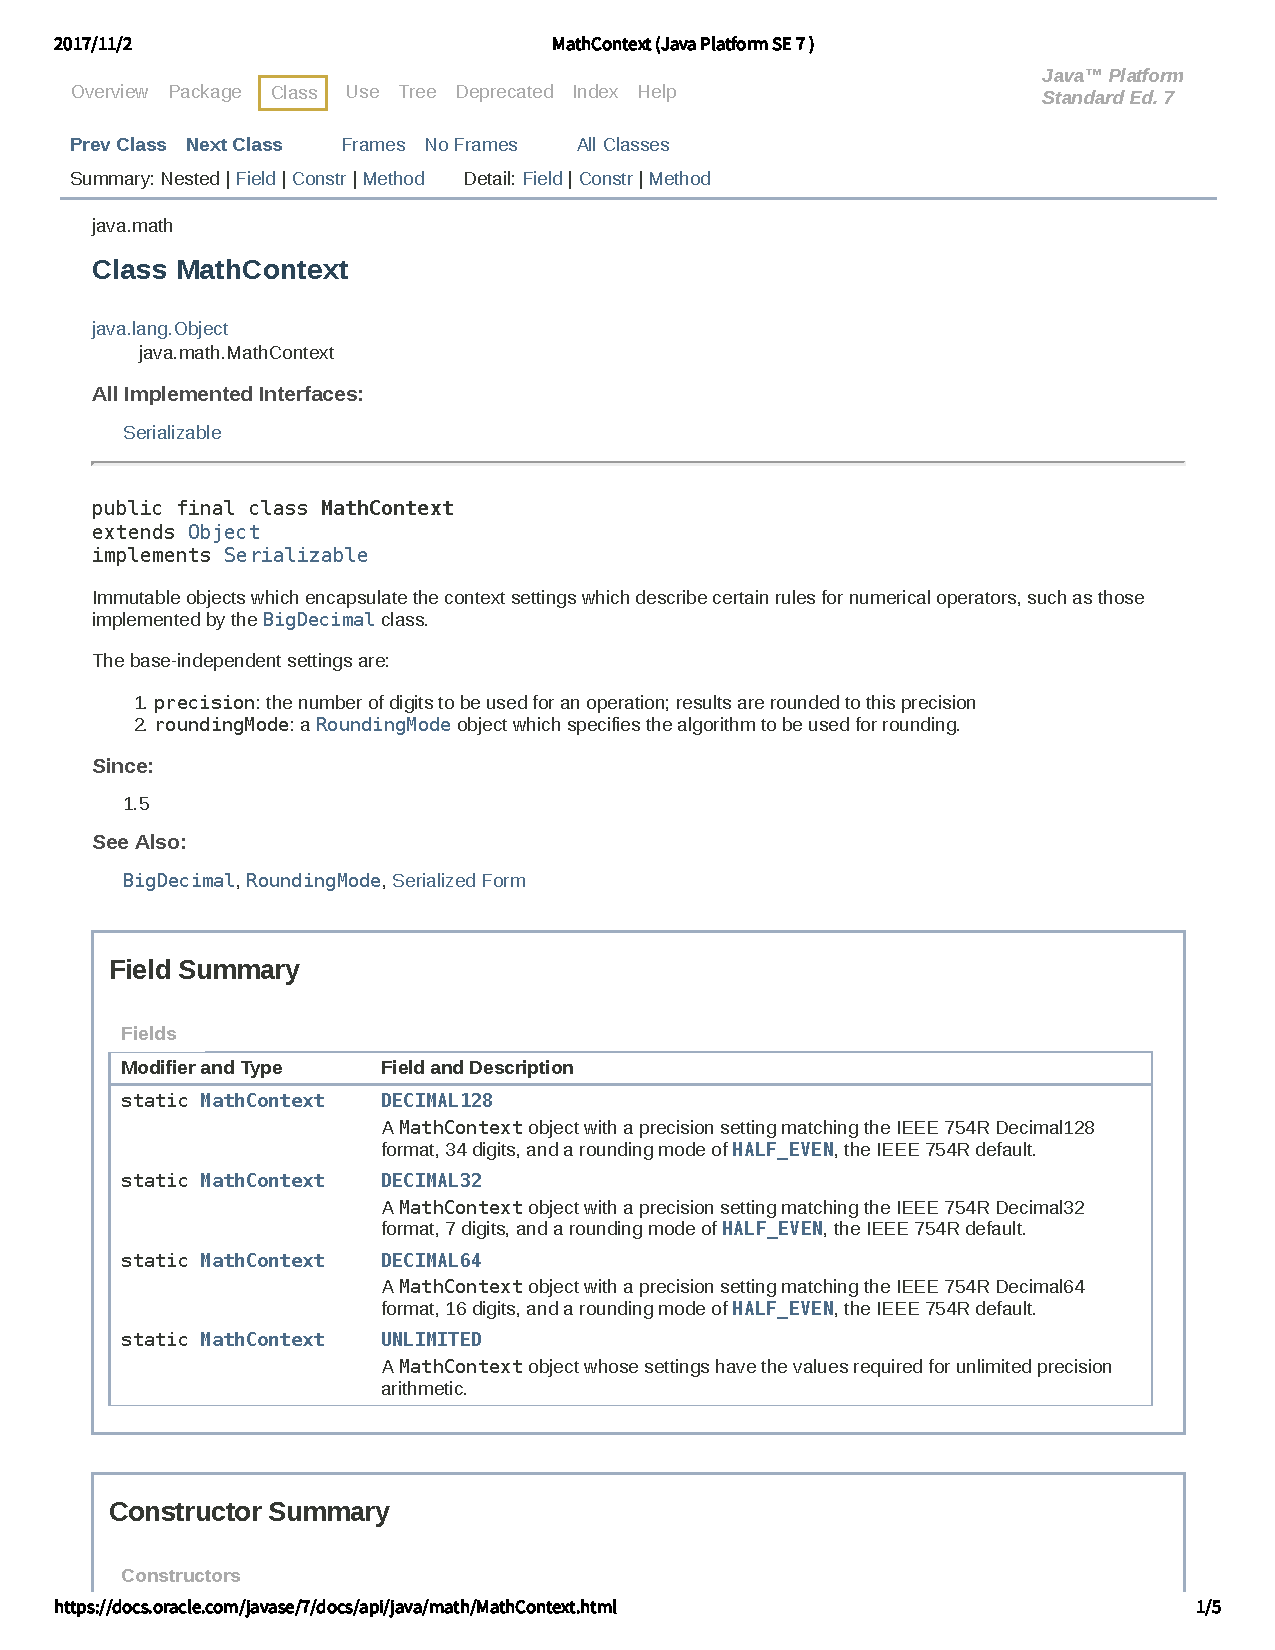
\includepdf[scale = 0.8,pages=1,pagecommand = \subsubsection{MathContext Class}]{MathContext-Class.pdf}
\includepdf[scale = 0.8,pages=2-5,pagecommand = {}]{MathContext-Class.pdf}
\newpage
% \subsubsection{RoundingMode Class}
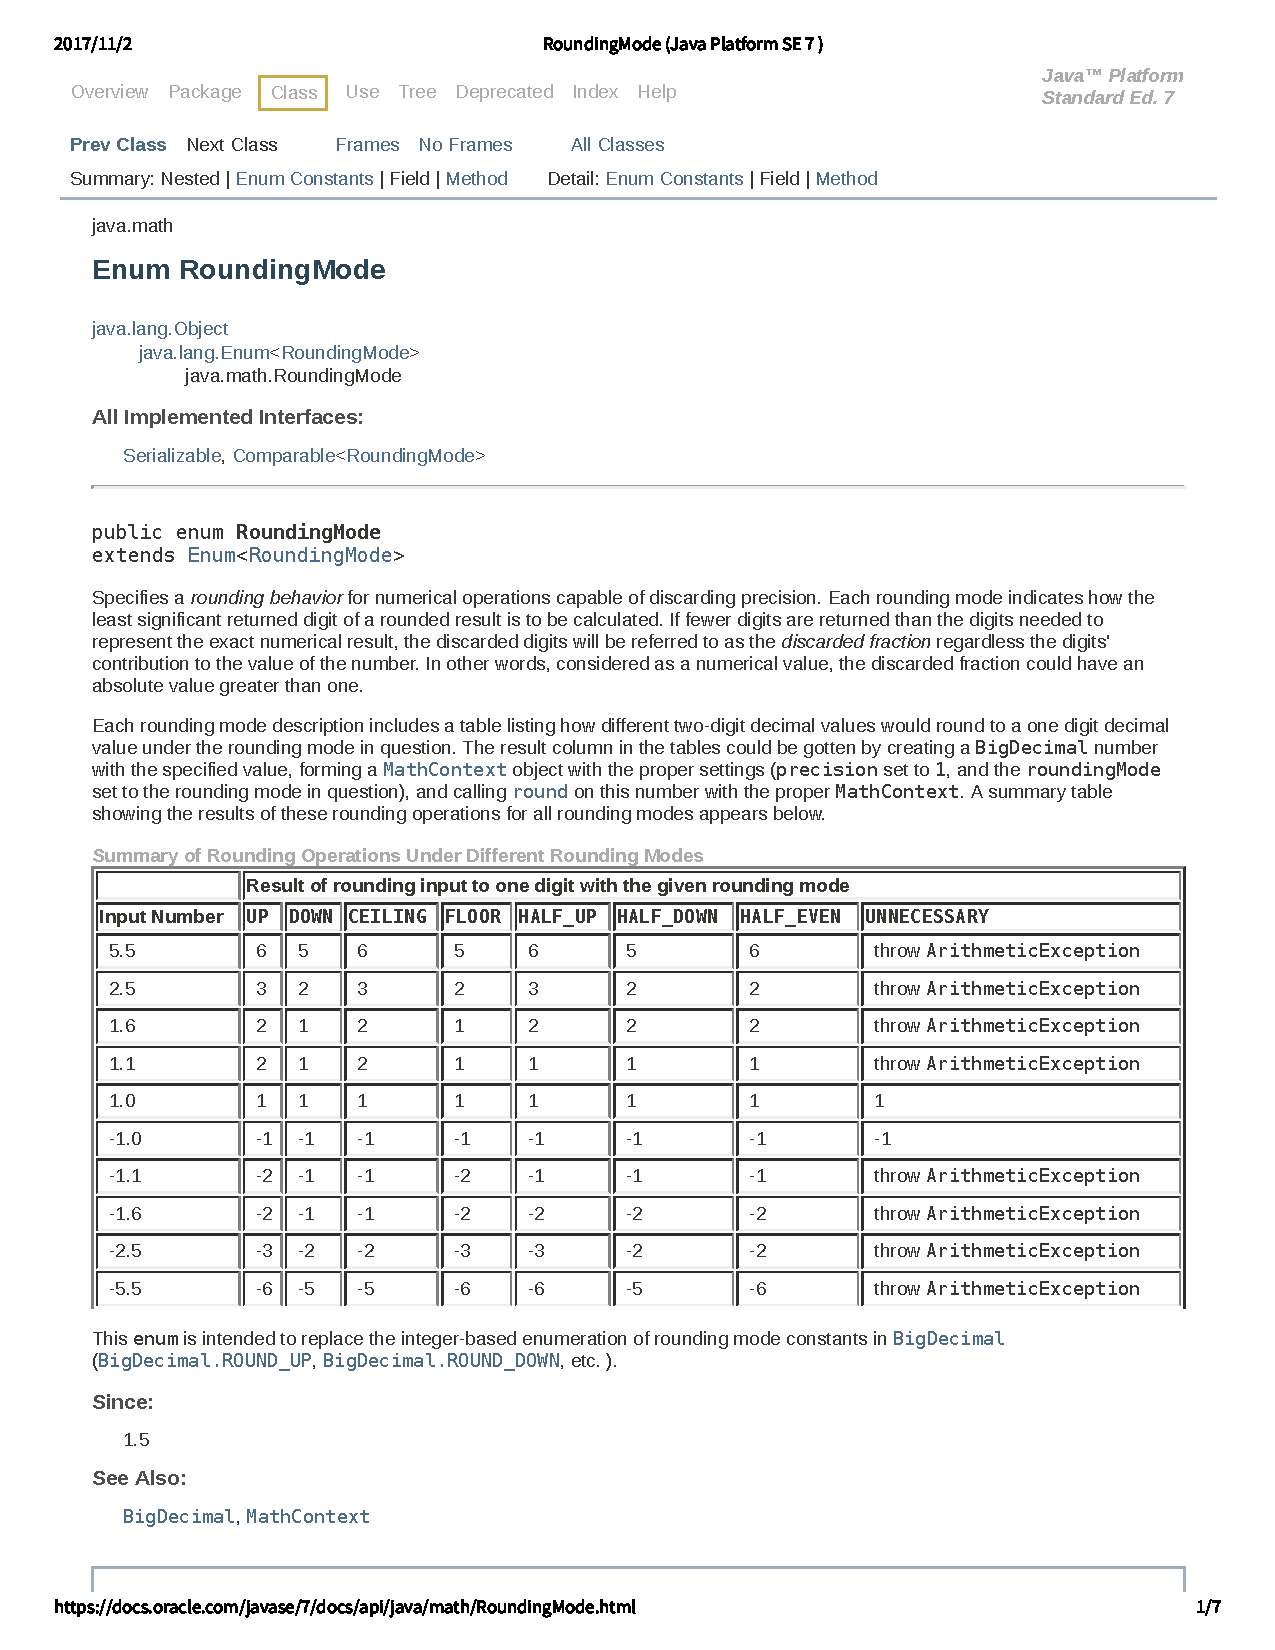
\includepdf[scale = 0.8,pages=1,pagecommand = \subsubsection{RoundingMode Class}]{RoundingMode-Class.pdf}
\includepdf[scale = 0.8,pages=2-7,pagecommand = {}]{RoundingMode-Class.pdf}
\newpage
% \subsubsection{String Class}
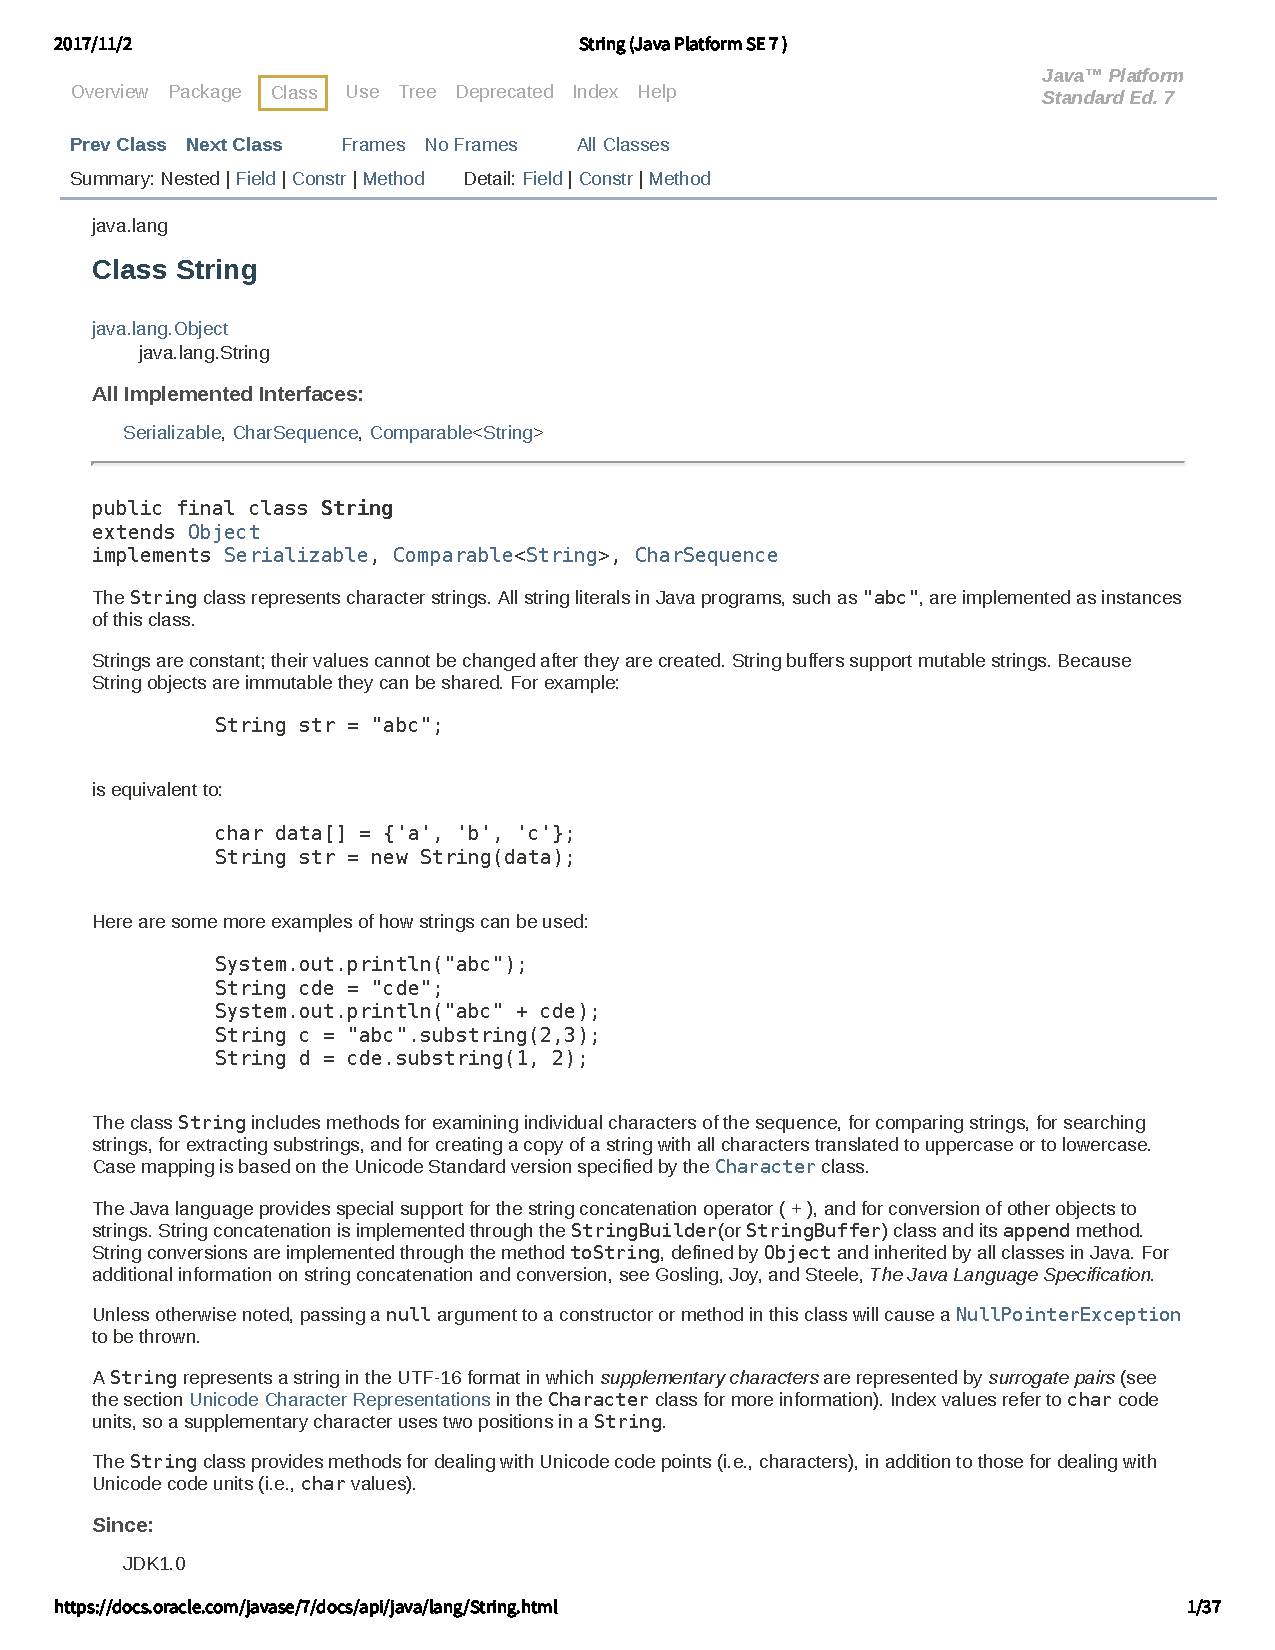
\includepdf[scale = 0.8,pages=1,pagecommand = \subsubsection{String-Class}]{String-Class.pdf}
\includepdf[scale = 0.8,pages=2-5,pagecommand = {}]{String-Class.pdf}
\newpage
\section{Emacs Configuration-Competition}
\emacscode{/Others/Competition.emacs}

\end{document}
